\FloatBarrier
\subsection{Database}

L'applicazione usa come supporto un database relazionale contenente i dati rigurdanti le aule dei vari edifici universitari e del personale.
\`E fondamentale però mettere in evidenza con un adeguato schema Entità/Relazione le tabelle utilizzate all’interno del progetto e create al fine del corretto funzionamento del 
sistema.

\begin{figure}[!htb]
\centering
\includegraphics[scale=0.60]{databaseER.png}
\caption{Diagramma E/R del database}\label{fig:database}
\end{figure}

Facendo riferimento alla figura \ref{fig:database}, descriviamo le entità fondamentali definite nel modello in esame:
\FloatBarrier
\begin{description}
\item[Room]\`e l'entit\`a principale. Essa contiene le informazioni riguardanti una specifica stanza di un determinato piano di un edificio. 
\item[Building]rappresenta l'edificio, caratterizzato da un numero univoco e dotato di un nome.
\item[Person]rappresenta il personale. Fondamentale per l'applicazione sono il ruolo di una persona (ad esempio docente e ricercatore) e le date di fine e inizio contratto lavorativo.
\item[OccupyRoom]associa una persona a una o pi\`u stanze diverse e  servir\`a ad ottenere una lista delle persone che occupano una stanza.
\end{description}

\FloatBarrier
\begin{figure}[!htb]
\centering
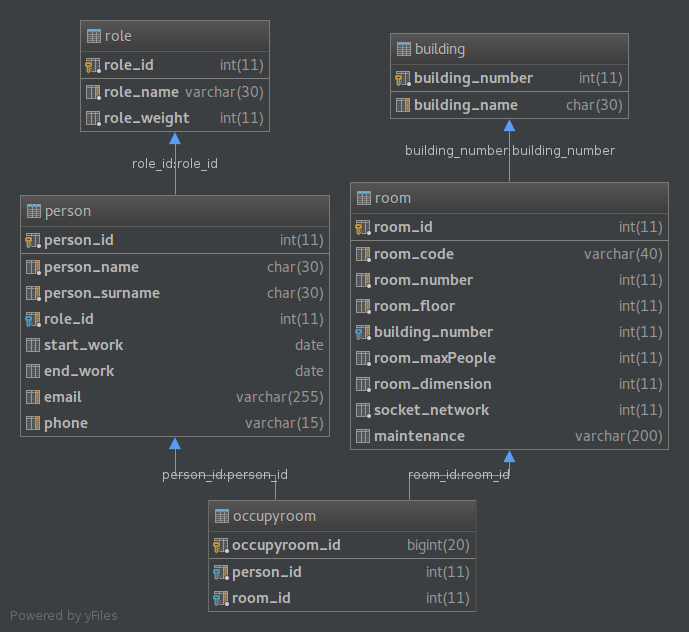
\includegraphics[scale=0.55]{diagram.png}
\caption{Modello Relazionale del database}\label{fig:databaseRelaz}
\end{figure}
\FloatBarrier
Dopo aver sviluppato il modello relazionale(figura \ref{fig:databaseRelaz}), tramite una metodologia bottom up, sono stati interfacciati oggetti Java con il database relazionale attraverso file di mappatura XML, uno per ogni classe che si vuole rendere persistente.\\ 

\begin{figure}[!htb]
\centering
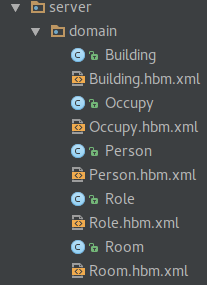
\includegraphics[scale=0.55]{packageMapping.png}
\caption{Package contenente i file di mappatura e le corrispondenti classi Java.}\label{fig:mappingPack}
\end{figure}
\FloatBarrier
Questi file di mappatura sono caratterizzati  dalle dualità classe-tabella e attributo-colonna.